\chapter{Исследовательская часть}

В данной части будет проведён сравнительный анализ последовательного и параллельного алгоритмов генерации кадра с использованием трассировки лучей.

\section{Технические характеристики}
Исследования проводились на устройстве со следующими характеристиками~\cite{macbook_spec}:
\begin{itemize}
	\item операционная система MacOS Tahoe 26.0.1 (25A362);
	\item процессор Apple M3, 8 ядер --- 4 производительных и 4 энергоэффективных;
	\item оперативная память 16 Гигабайт, LPDDR5;
\end{itemize}
Во время замеров времени ноутбук был подключён к зарядному устройству. Никакие пользовательские задачи в фоне не выполнялись. Оптимизация компилятора выключена флагом -o0~\cite{compilator_level_optimize}.

\section{Временя выполнения последовательной и параллельной реализации алгоритма}

Была исследована зависимость времени выполнения последовательной и параллельной реализации алгоритма от количества объектов на сцене. Для каждого значения варьируемого параметра измерение проводилось 100 раз, полученные значения времени суммировались, после чего усреднялись. Результаты исследование приведены в таблице~\ref{tab:res_1} 

\begin{table}[H]
	\centering
	\caption{Сравнение времени выполнения реализаций последовательного и параллельного алгоритмов}
	\label{tab:res_1}
	\begin{tabular}{|p{5cm}|p{5.65cm}|p{5.05cm}|}
		\hline
		\textbf{Количество объектов} & \textbf{Время выполнения последовательной реализации, мс} & \textbf{Время выполнения параллельной реализации, мс} \\
		\hline 2  & 172 & 180 \\
		\hline 4  & 197 & 201 \\
		\hline 6  & 217 & 221 \\
		\hline 8  & 235 & 239 \\
		\hline 10 & 252 & 261 \\
		\hline 12 & 268 & 272 \\
		\hline 14 & 289 & 294 \\
		\hline 16 & 310 & 315 \\
		\hline 18 & 326 & 331 \\
		\hline
	\end{tabular}
\end{table}

На рисунке~\ref{fig:risunok_6} изображены графики зависимости времени выполнения алгоритма от количества объектов, попадающих в кадр.
\begin{figure}[H]
	\centering
	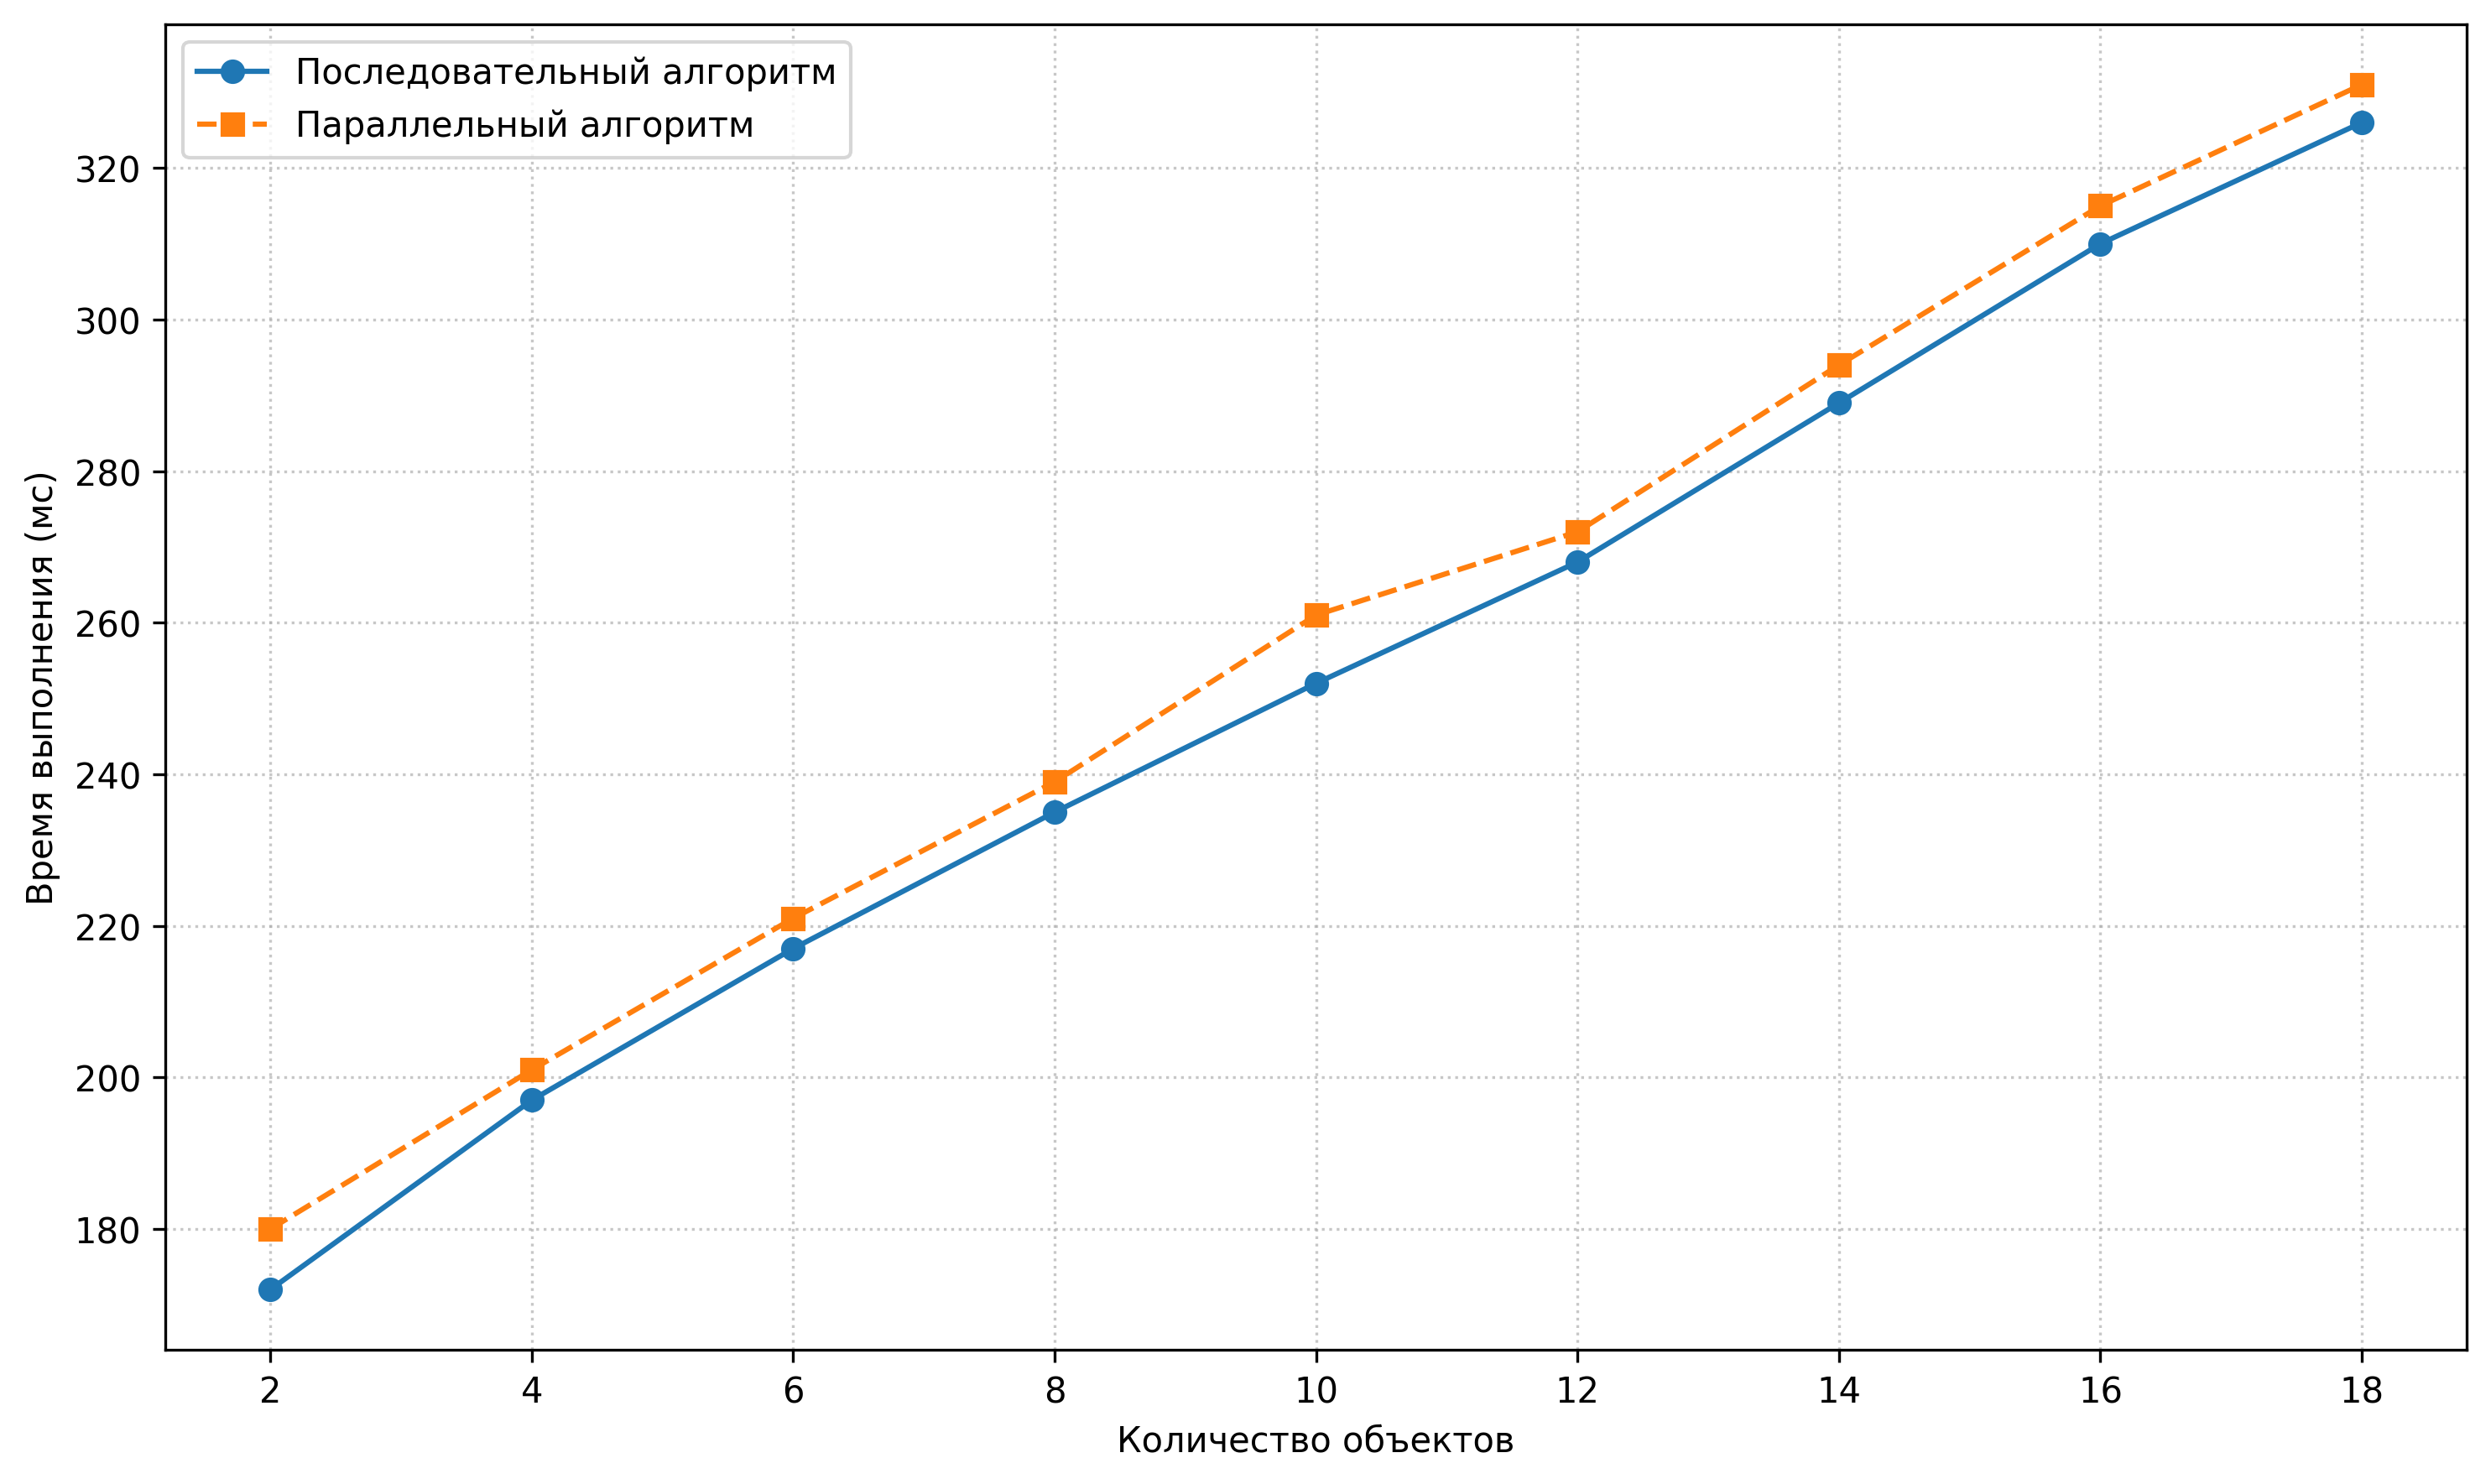
\includegraphics[width=1\textwidth]{images/AA4_1.png}
	\caption{Графики зависимости времени выполнения реализации алгоритма от количества объектов}
	\label{fig:risunok_6}
\end{figure}

При использовании одного рабочего потока последовательный алгоритм в среднем превосходит параллельный по производительности на 10\%. Данное различие обусловлено более простой логикой последовательной реализации, в то время как параллельная версия несёт накладные расходы, связанные с организацией и управлением пулом потоков.

\section{Исследование зависимости времени выполнения реализации алгоритма от числа потоков}

Была исследована зависимость времени выполнения параллельного алгоритма генерации кадра от количества рабочих потоков и количества объектов, попадающих в кадр. Результаты исследования приведены в таблице~\ref{tab:res_2}

\begin{table}[H]
	\centering
	\caption{Время выполнения реализации параллельного алгоритма в зависимости от количества потоков}
	\label{tab:res_2}
\begin{tabular}{|>{\centering\arraybackslash}p{4cm}|*{8}{>{\centering\arraybackslash}p{1.15cm}|}}
	\hline
	\makecell{\textbf{Количество}\\\textbf{потоков}} & 
	\multicolumn{8}{c|}{\makecell{\textbf{Количество видимых объектов}}} \\
	\cline{2-9}
	& 1 & 2 & 3 & 5 & 10 & 15 & 20 & 25 \\ 
	\cline{2-9}
	& \multicolumn{8}{c|}{\makecell{\textbf{Время выполнения, мс}}} \\
	\hline
	1  & 85 & 103 & 113 & 138 & 202 & 252 & 304 & 386 \\
	\hline
	2  & 47 & 52 & 59 & 71 & 100 & 144 & 178 & 211 \\
	\hline
	4  & 27 & 29 & 32 & 40 & 56 & 73 & 89 & 105 \\
	\hline
	8  & 21 & 22 & 25 & 30 & 40 & 63 & 82 & 98 \\
	\hline
	16 & 23 & 24 &  27 & 35 & 45 & 52 & 66 & 95 \\
	\hline
	24 & 24 & 25 & 29 & 32 & 40 & 50 & 60 & 97 \\
	\hline
	32 & 26 & 27 & 28 & 32 & 42 & 49 & 66 & 96 \\
	\hline
	64 & 26 & 28 & 27 & 31 & 44 & 51 & 62 & 98 \\
	\hline
	128 & 27 & 29 & 30 & 34 & 43 & 52 & 61 & 99 \\
	\hline
\end{tabular}
\end{table}

На рисунке~\ref{fig:risunok_7} приведены результаты замеров процессорного времени выполнения реализации параллельного алгоритма для разного числа потоков.
\begin{figure}[H]
	\centering
	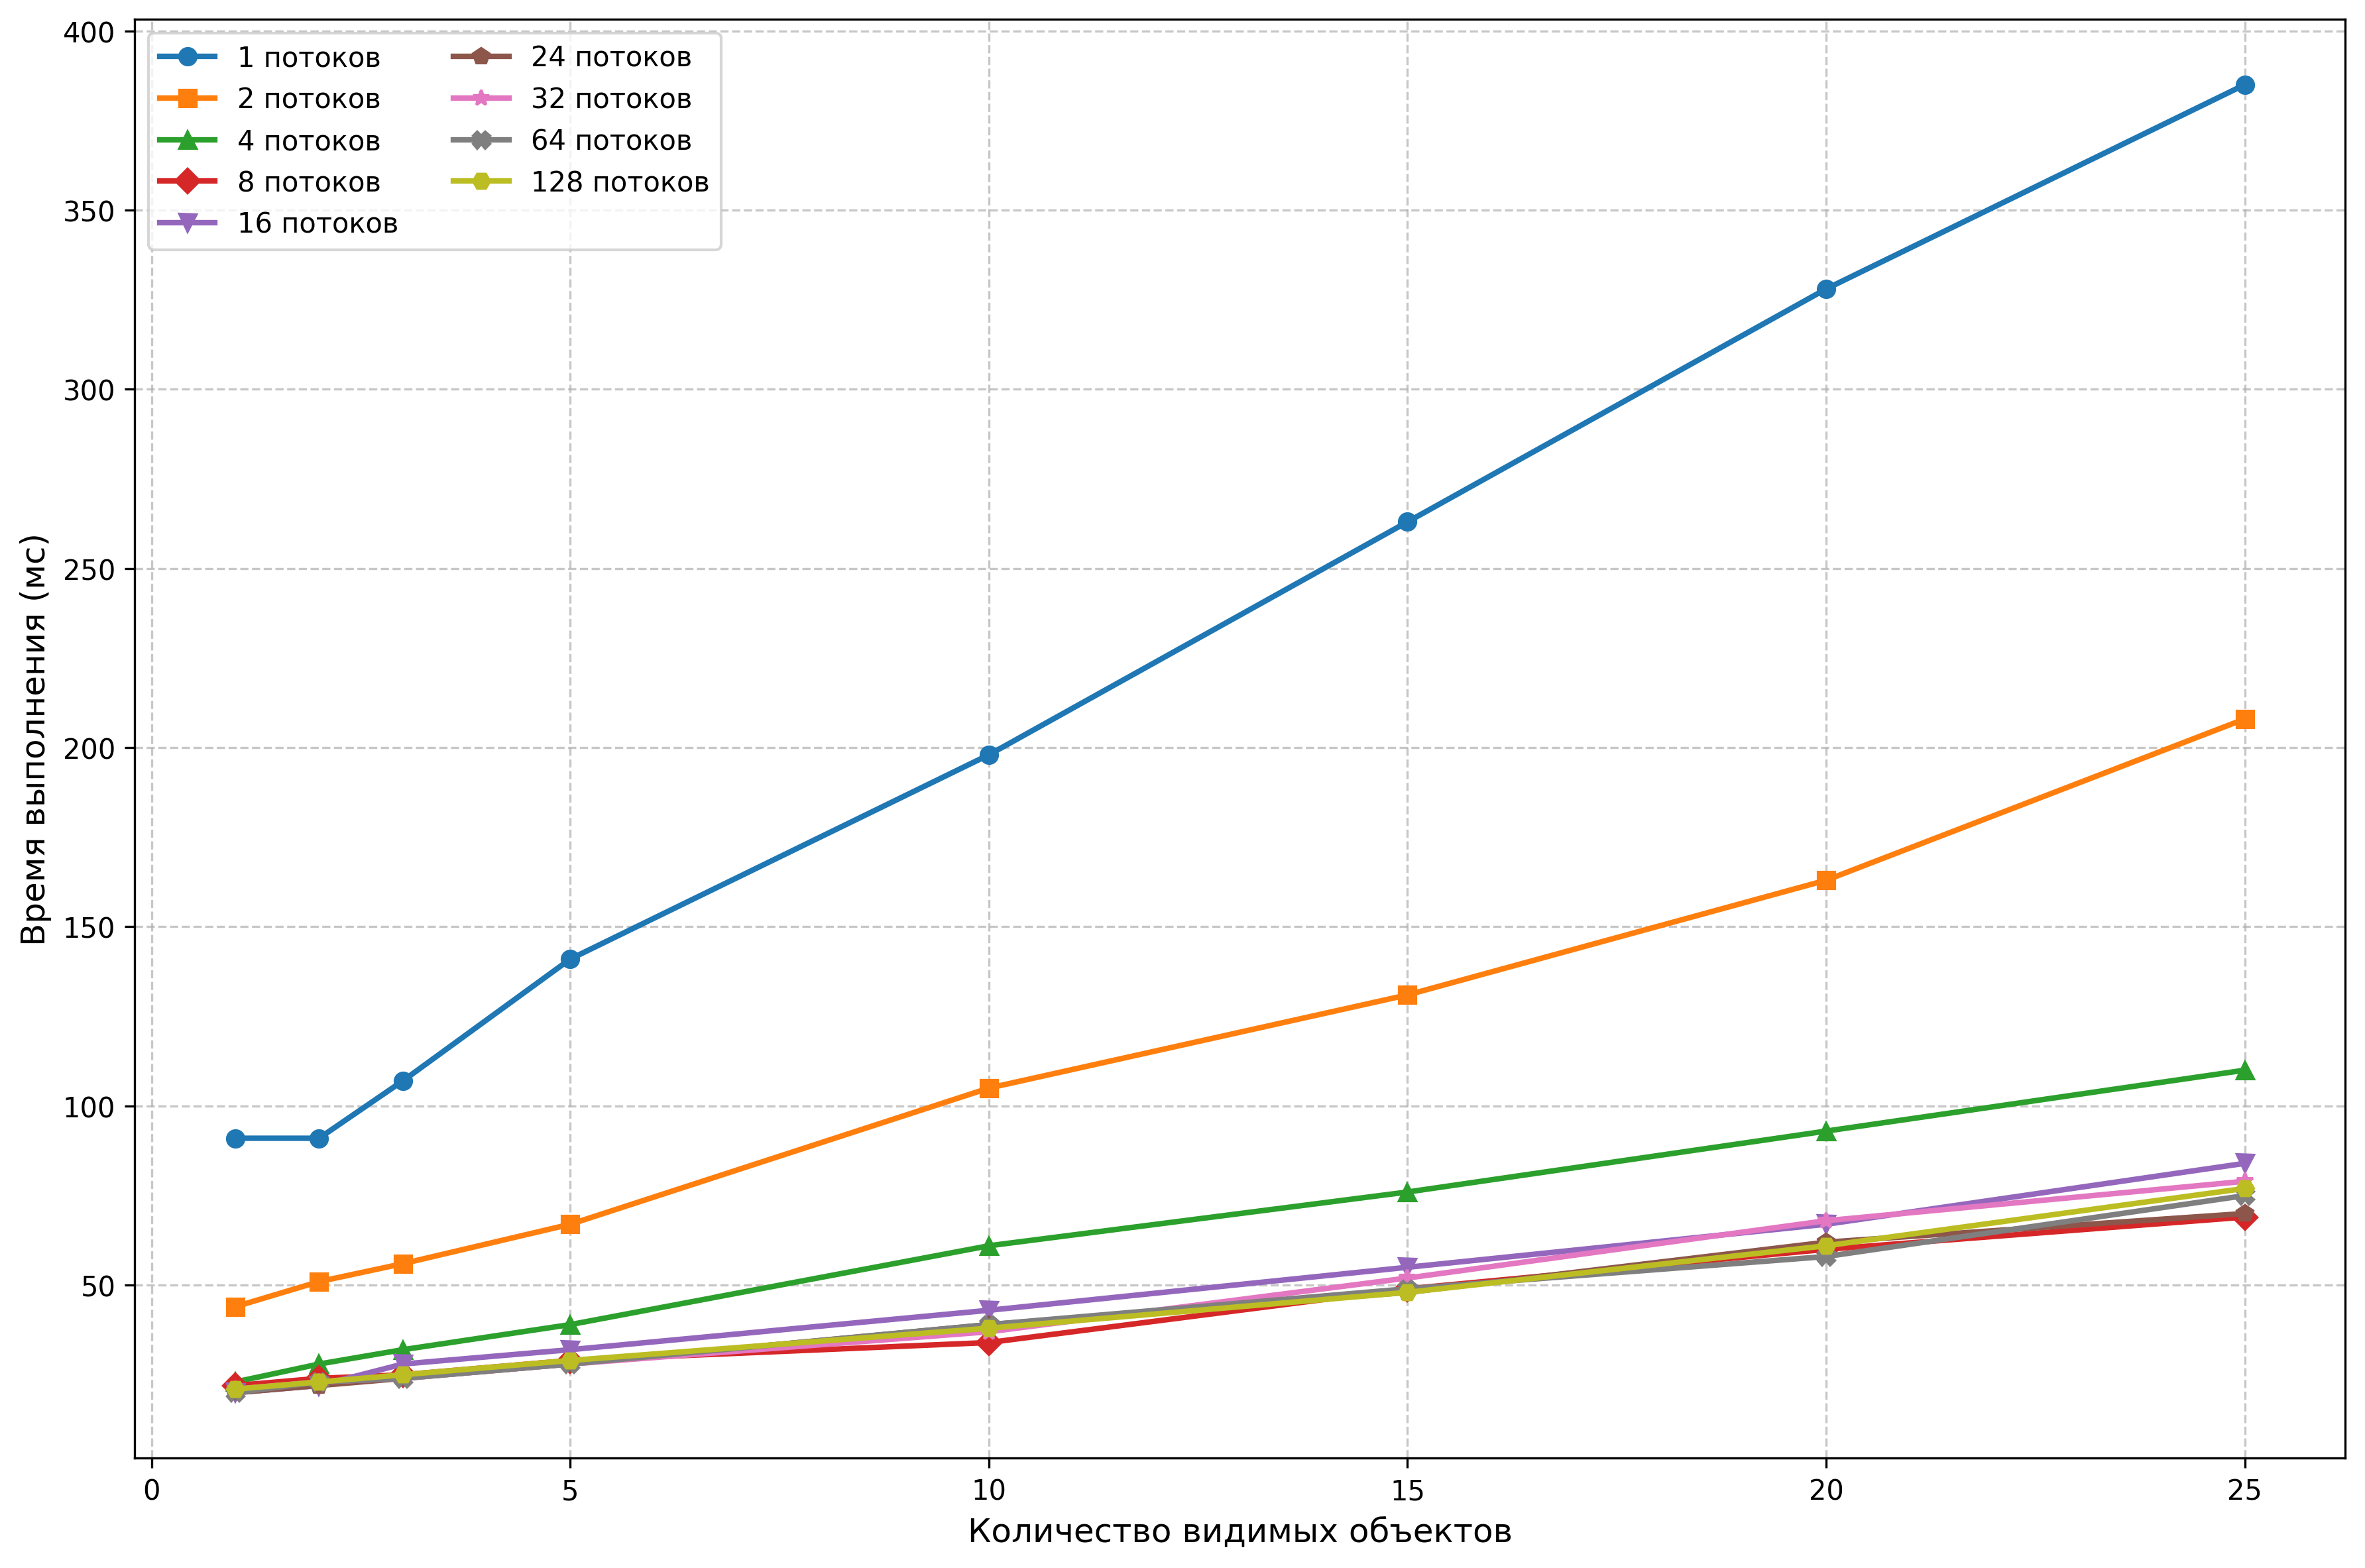
\includegraphics[width=1\textwidth]{images/AA4_2.png}
	\caption{Время выполнения реализации параллельного алгоритма в зависимости от количества потоков}
	\label{fig:risunok_7}
\end{figure}

\section*{Вывод}

В данной части представлены технические характеристики используемой вычислительной системы и результаты исследования, проведённого на ней. По итогам анализа полученных данных сделаны следующие выводы.

\begin{itemize}
	\item Время выполнения последовательной реализации алгоритма и параллельной реализации с одним рабочим потоком практически совпадает при любом количестве видимых объектов. Это свидетельствует о том, что создание и запуск одного потока сопряжены с минимальными накладными расходами.
	\item С ростом числа потоков время выполнения уменьшается. Это заметно до 8 потоков, после чего время выполнения начинает расти. Это связано с тем, что при превышении аппаратных возможностей процессора накладные расходы на управление потоками (создание, переключение контекста) начинают преобладать над выгодой от распараллеливания.
	\item Наилучшее время выполнения параллельного алгоритма достигается при использовании 8 потоков. Используемый процессор обладает 8 физическими и 8 логическими ядрами.
	\item При увеличении количества видимых объектов время выполнения как последовательной, так и параллельной реализации растёт линейно.
\end{itemize}

\clearpage
